\documentclass[12pt]{article}
\usepackage{graphicx}

\author{Samuel Young}
\title{Exam II question II}
\date{Thursday November 24th, 2018}
\begin{document}
\maketitle

\part{2.A}
   There are just about 72 possible ALL and AML data point within the data set. There are a total 47 ALL in the dataset and 25 of the AML in the same data set. So the genes are the rows and the columns are the patients. So first I did a wordcount on the file to see how many rows there are and then minus the 7219-1 to get a close approximation to the numbers there are 72* 7218 differnet genes to look at for the data set.
 
  \part{2.B}
                  I orignial thought that there were at least 500-1000 of these genes had a greater than or equal to 2.000 p-value with a degree of freedom of 60, It was any assumption, made based on t-chart that I made base on the data that was given. But considering there are to different sigigincat factor that can still be held true.Isn't the t-value a close approxiamation of where the data lie with a standard devations lie.That is the reason why based upon the graph and the intial t-value with a siginificates of $\alpha=.05$ is super close to a significants of 2 standard deviations form the value.It was solely base on one data set when what I should have of been doing it is basing upon both data sets and I should of tried to find a collective average of all the sets then taken that and found the t-values based on the siginigcants. That were given and that would of increased the p-value for both charts. Now based on those two differing level instead of using one. It was  appearentlty closer to 2072 genes a within this p-value range I got that was based on  the exact way you put it $(.03=(\frac{2072}{7218*72})*100))$ is each to 28 percent of all the lines has a siginificant. What is 30 precent a close apporximate to 28 precent. A p-value is a value that is a statistcal test that is shown with $1 - \int_{-\infty}^{cv} \mathrm{f(t)}$.
\part{2.C}
      In this part where were told to make a any algorthim using permutaion.py. In which, I removed th    e first time you called the absulote value and got half that exact same amount. -1.51 as the value f    or the oringal so then you have to do that absolute value of that inorder for you to determine that     the grah is in representation of both sides. 3.02 when you keep the absolute value. but because you     are looking at both tails of the graph in this one you will obtain a more bell-like graph in the cas    e that now you are trying to find all the values that are outside of the graph in which when  you ru    n this like 3-5 times you obtain an estimated 968 out of all the genes that are similar.
  \part{2.D}
                  I was able to obtain a graph but it appears to be right skewed base on the fact that it is only a one sided graphical representation of the data. With using only genes any number of list to generate this graph  as any input.
                  \begin{figure}
                  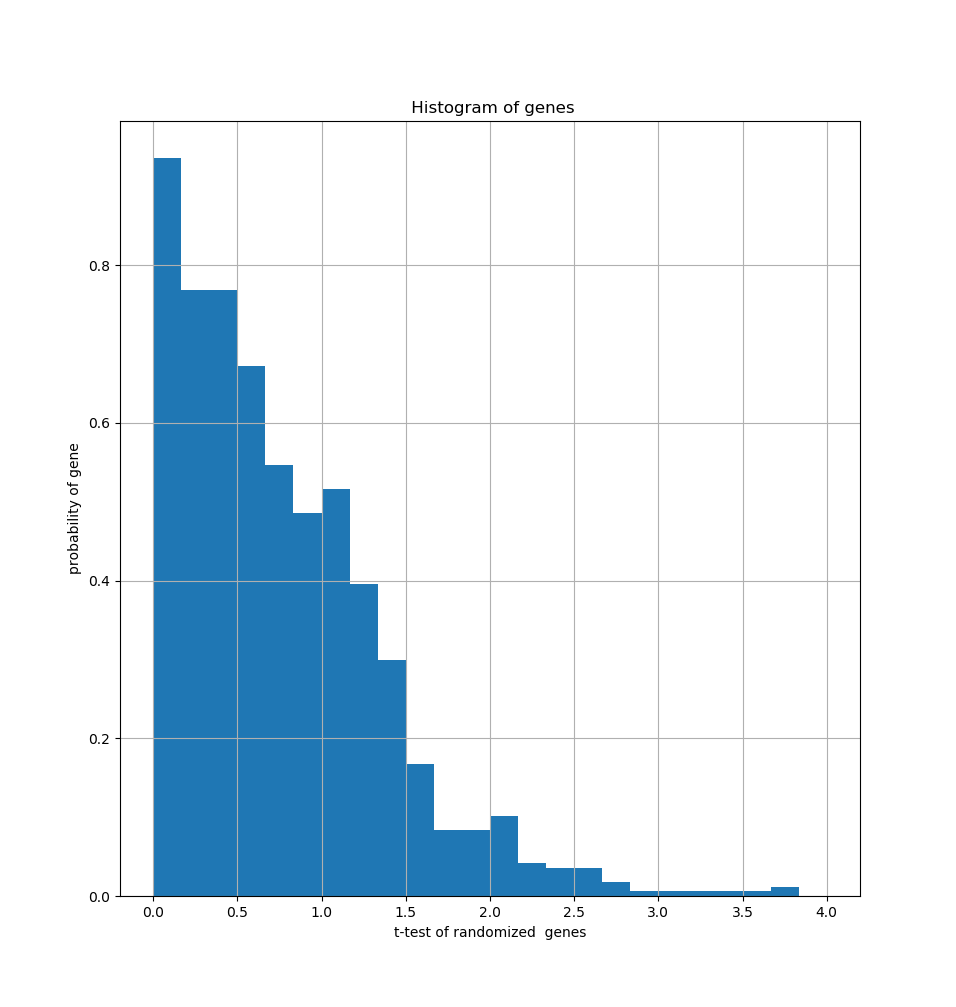
\includegraphics[width=\linewidth]{./Figure1.png}
                  \caption{A one side permutantion test with a graphical reperesntation of a bell-like     curve.}
                  \label{fig:graph1}
                  \end{figure}
                   This graph \ref{fig:graph1} show that the absolute value when taken as the first number.
\part{2.E}
   So with with the permuatation data that I randomly shuffled around I was able to get much more clos    er to the .05 precent with a few tweaks to the intial values. Unforunately, my numbers do randomly s    hift around alot so there is always a chance of obtaining a prefect number,1.962, because the value     will variey 1.565 p-value closer and then there is also a chance of obtain a 3.765 p-value father aw    ay form the table. Another weird thing that i realized about my program is that It more closer to 10000 times rather then a thousand fold.
\end{document}

